\section{MD5}\index{хеш-функция!MD-5|(}
\selectlanguage{russian}

Одна из наиболее популярных в прошлом, но криптографически нестойкая хеш-функция MD5 (от \langen{message digest 5}), разработана Рональдом Ривестом (\langen{Ronald Linn Rivest}) в 1991 году как развитие хеш-функии MD4 и представлена как RFC 1321 в апреле 1992 года (\cite{rfc1321}).

MD5 разрабатывалась как криптографически-стойкая хеш-функция с длиной выходного блока 128 бит. Исходный текст сначала дополняется до целого числа обрабатываемых блоков по 512 бит (рис.~\ref{fig:md5-padding}).

\begin{figure}[htb]
    \centering
    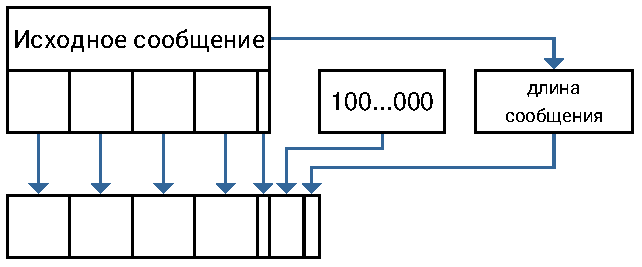
\includegraphics[width=0.95\textwidth]{pic/md5-padding}
    \caption{Дополнение открытого текста до целого числа 512-битовых блоков в хеш-функции MD5}
    \label{fig:md5-padding}
\end{figure}

\begin{itemize}
  \item Дополнение (паддинг). Исходное сообщение рассматривается как последовательность бит и дополняется сначала единичным битом \texttt{1}, а далее нулевыми битами \texttt{{000}\dots{000}} до тех пор, пока остаток от деления сообщения в битах по модулю 512 не будет равен 448.
  \item Добавление длины сообщения. Длина исходного сообщения в битах (до дополнения) добавляется в виде 64-битового значения к обрабатываемому тексту. Если текст имеет длину больше, чем $2^{64}$ бита, используется остаток от деления длины на $2^{64}$.
\end{itemize}

Далее обрабатываемый текст разбивается на целое число 512-битовых блоков $M_i$ и выполняется последовательное вычисление хеш-функции по итеративной формуле:
\[\begin{array}{l}
H_i = f ( H_{i-1}, M_i ),\\
H_0 = \text{IV}.\\
\end{array}\]

В качестве начального значения $H_0 = \text{IV}$ выступает конкатенация заданных в стандарте 16-ричных последовательностей:
\[\begin{array}{l}
A = \text{01} ~ \text{23} ~ \text{45} ~ \text{67},\\
B = \text{89} ~ \text{ab} ~ \text{cd} ~ \text{ef},\\
C = \text{fe} ~ \text{dc} ~ \text{ba} ~ \text{98},\\
D = \text{76} ~ \text{54} ~ \text{32} ~ \text{10}.\\
\end{array}\]

\begin{figure}[htb]
    \centering
    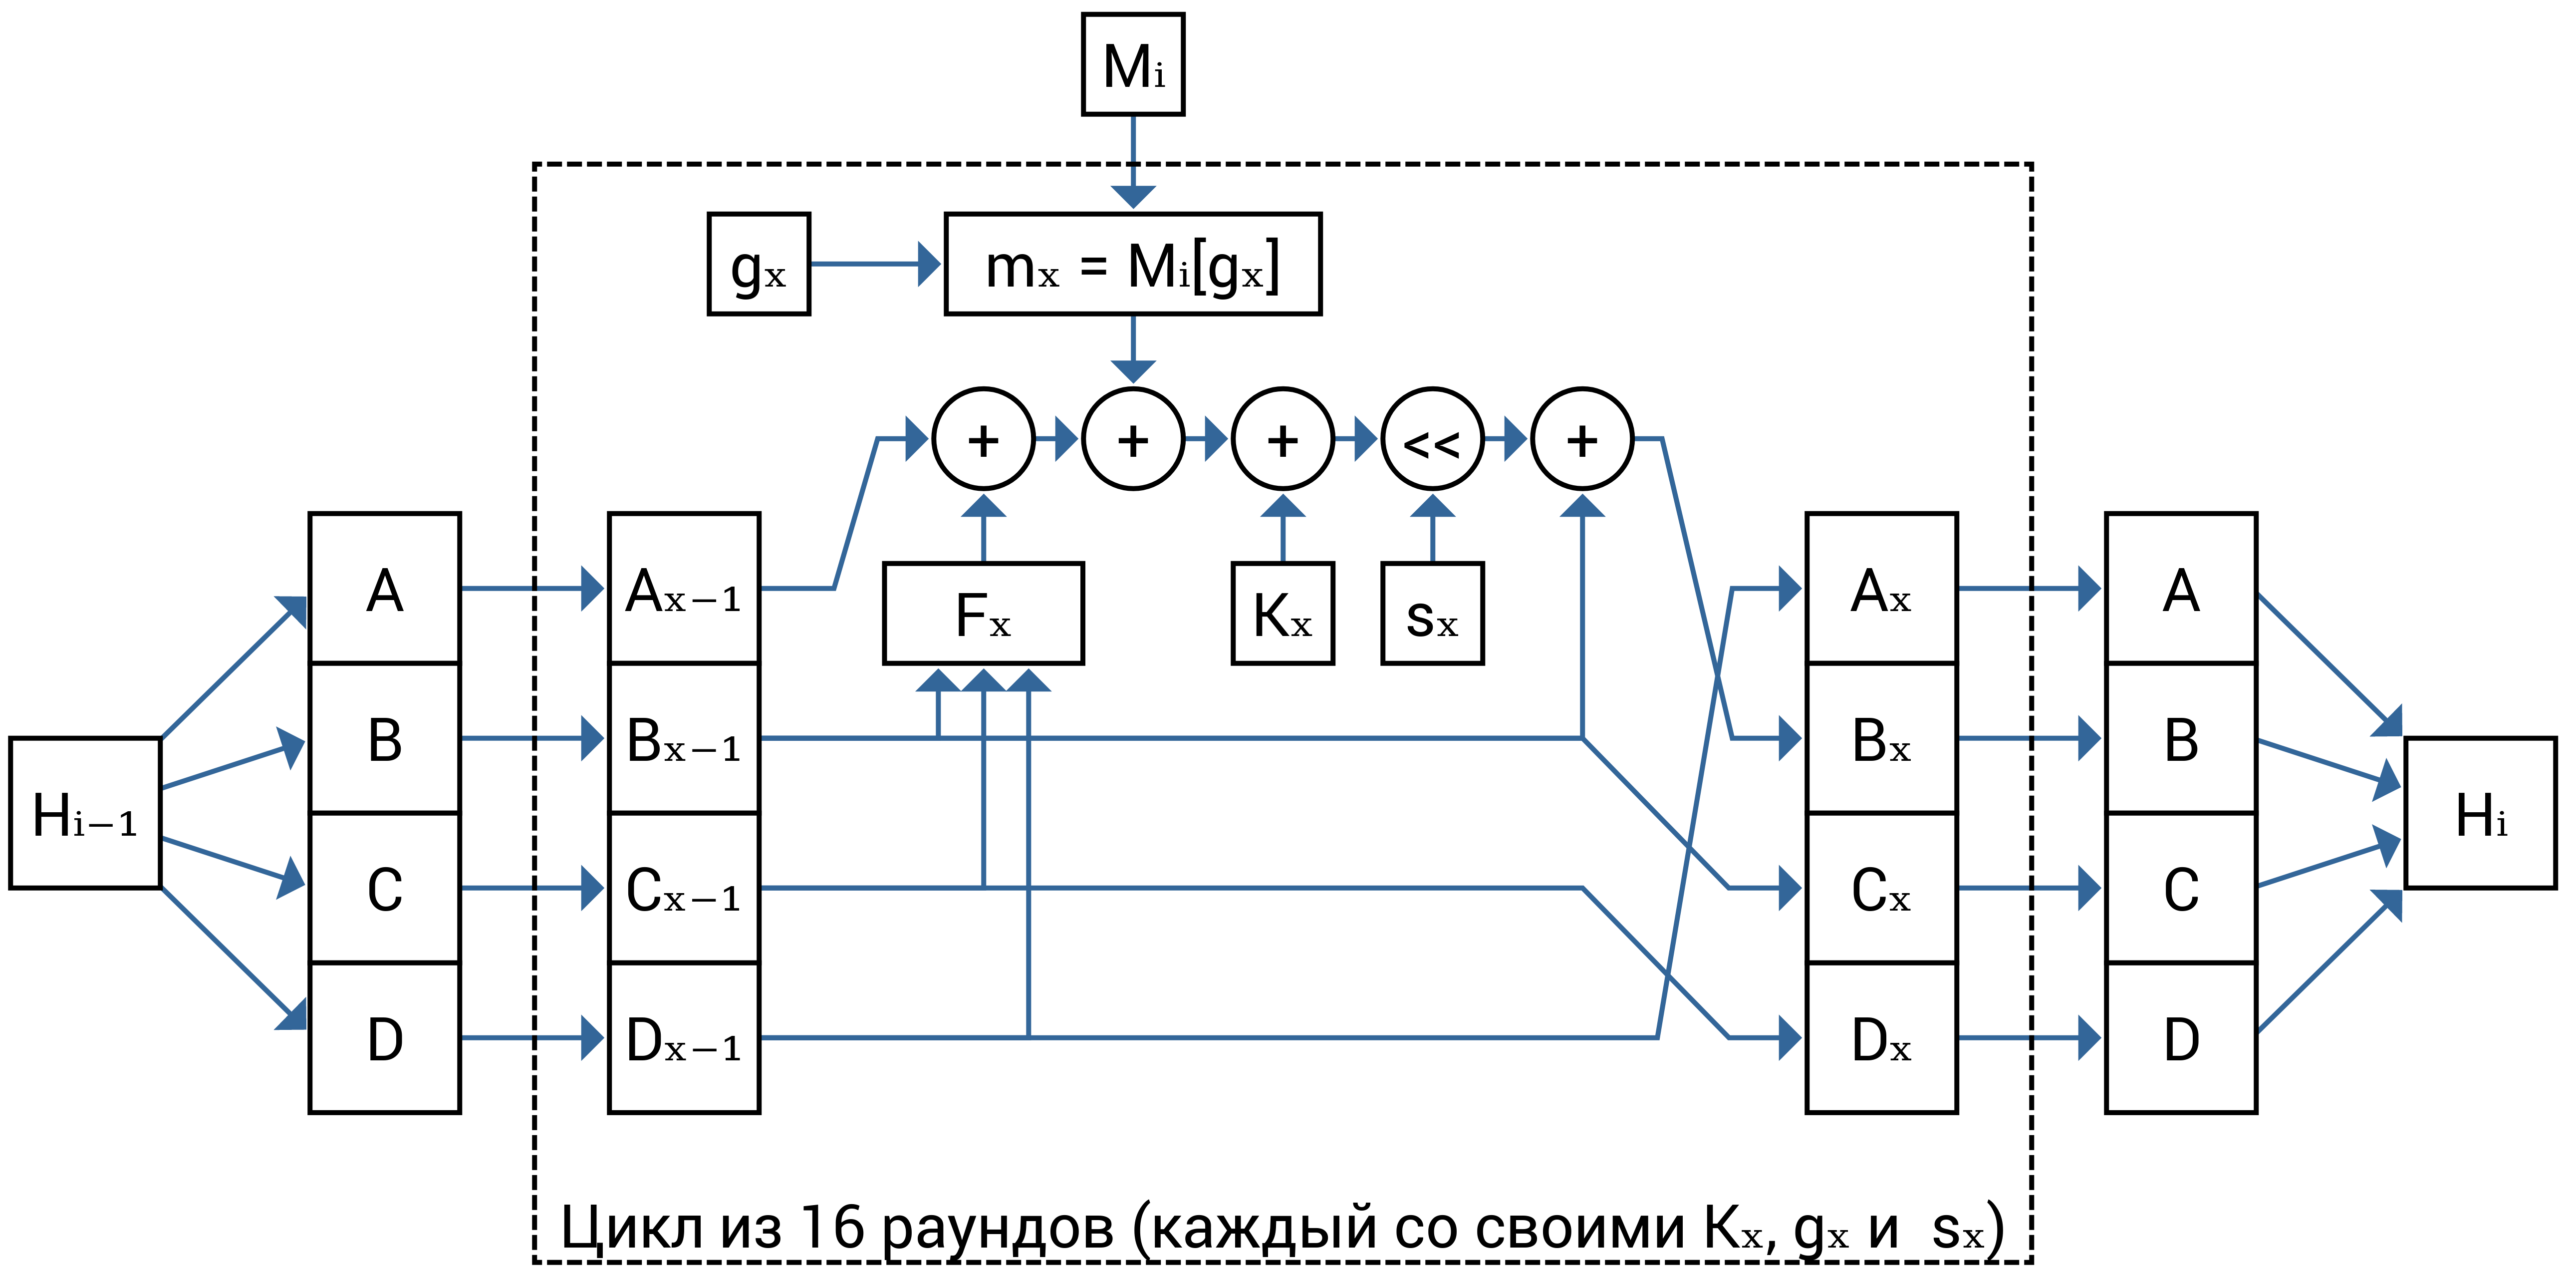
\includegraphics[width=\textwidth]{pic/md5-round}
    \caption{Один раунд преобразования текста в хеш-функции MD5}
    \label{fig:md5-round}
\end{figure}

Каждый из этапов вычисления $H_i = f ( H_{i-1}, M_i )$ состоит из 16 раундов (рис.~\ref{fig:md5-round}), на котором выполняется преобразование четырёх 8-битовых блоков $A, B, C, D$. Основное преобразование выполняется с первым из блоков $A$ (который в конце раунда становится блоком $B$, и далее по кругу, что делает процедуру чем-то похожей на схему Фейстеля). К значению $A_{x-1}$ из результата предыдущего раунда (или предыдущего блока, если это первый раунд) прибавляется значение нелинейной функции $F(B, C, D)$, числовое значение некоторого байта из $M_i$ (индекс байта определяется константой $g_x$), значение раундового <<ключа>> $K_x$. Полученное значение сдвигается влево на количество бит, определяемое ещё одной константой раунда $s_x$, арифметически складывается со значением блока $B_{x-1}$ и считается новым значением блока $B_x$. Остальные блоки циклически сдвигаются без изменений ($B_{x-1} \to C_x$, $C_{x-1} \to D_x$, $D_{x-1} \to A_x$).

Вид нелинейной функции $F$ и значения констант $g_x$, $K_x$, $s_x$ отличаются для каждого из 16 раундов и заданы в описании на хеш-функции. 

Значения $A, B, C, D$ результата обработки самого последнего блока $M_i$ конкатенируются и считаются результатом вычисления хеш-функции.

Уже на примере хеш-функции, предложенной в 1991 году, можно увидеть общие свойства, которые присущи большей части современных хеш-функций.

\begin{itemize}
  \item Во-первых, разбиение исходного текста на блоки равной длины и дополнение последнего блока дополнительными значениями (для финального преобразования), возможно включая длину исходного открытого текста или какую-либо простую функцию от всех блоков сообщения.
  \item Во-вторых, наличие некоторой функции преобразования $H_i = f ( H_{i-1}, M_i )$, которую можно рассматривать как фактически функцию шифрования некоторого блочного шифра. Но при этом в качестве шифруемого текста выступает результат хеширования предыдущего блока $H_{i-1}$, а блок исходного хешируемого сообщения $M_i$ выступает в качестве ключа шифрования. От стойкости данного шифра зависит возможность (при известных $H_{i-1}$ и $H_{i}$) восстановить <<ключ шифрования>>, то есть часть исходного сообщения, особенно если оно короткое (меньше одного блока, то есть фактически осуществить атаку на восстановление прообраза.
\end{itemize}

В будущем подобный подход будет формализован более явно, в том числе с помощью описания конструкций Меркла~---~Дамгарда и Миагучи~---~Пренеля (см. раздел~\ref{section-stribog} про хеш-функцию <<Стрибог>>).

\index{хеш-функция!MD-5|)}